\documentclass{article}
\usepackage[utf8]{inputenc}
\usepackage{cite}
\usepackage{graphicx}
%\usepackage{mathtools}
\usepackage{amsmath}
%\usepackage{mathptmx}
%\usepackage{amsfonts}
%\usepackage{amssymb}
\usepackage{url}
\usepackage{color}

%\renewcommand*\rmdefault{dayroms}
\setlength\parindent{0pt} % Geen /newline gezeik ;)
%\renewcommand{\familydefault}{\ttdefault}
\renewcommand*\sfdefault{cmss}

\newcommand{\horrule}[1]{\rule{\linewidth}{#1}}
\title{	
	\normalfont \normalsize
	\horrule{2pt} \\[0.25cm]
	\huge Hardware Security: JavaCard \\
	\large Design document - petrol allowance \\
	\large Radboud University Nijmegen\\
	\horrule{0.5pt} \\[0.125cm]
}
\author{\normalsize \textbf{Group 2:} Wouter Kuhnen (s4081420), Wouter van Kranenburg (s4319176),\\\normalsize Ye Myat Kaung (s4460677),  Stephanie Silvius (s4380479)}

\date{\today}

\begin{document}


\maketitle
\newpage
% Chapters
\tableofcontents
\newpage
\section{Terminology and abbreviations}
The following terminology and abbreviations will be used throughout this document. 
    \begin{center}
        \begin{tabular}{| l | p{8cm} |}
            \hline
            $PRS$ & Petrol Rationing System\\\hline
            $IT$ & Personalisation terminal, used for the initialisation of the petrol card \\\hline
            $PT$ & Petrol terminal \\\hline
            $CT$ & Charging terminal \\\hline
            &\\\hline
            \textbf{For the protocols:} &\\\hline
            $ENC_{SK}\{X\}$ & encryption function for X with symmetric key (SK) agreed to by both parties\\ \hline
            $SIG[X]_{priv}$ & signing function for X with private key of sender \\ \hline
            $[X]_{pub}$ & encryption function for X with a public key of the sender \\ \hline
            $certificate_{X}$ & certificate of X \\ \hline
            $pub_{X}$ & public key of X \\ \hline
            $priv_{X}$ & private key of X  \\ \hline
            $ID_{X}$ & Identification (ID) number of X \\ \hline
            $SK$ & Symmetric Key \\ \hline
            $Verify(cert)$ & Certificate Verification function\\ \hline
            $Log()$ & Logging function to keep track of transactions \\ \hline
            $T$ & Terminal (charging/petrol) \\ \hline
            $PC$ & Petrol Card \\ \hline
            $BE$ & Back-end \\ \hline
            $VTS$ & Valid timestamp until certificates are considered untrusted (24Hours from the time the CVR was requested) \\ \hline
            $TS$ & Timestamp \\ \hline
            $Certs$ & List of certificates that are valid and or revoked \\ \hline
            $CVR$ & Certificate Validity Request function \\ \hline
            $PIN$ & PIN number \\ \hline
            $PIN_{AUTH}$ & Boolean response to indicate validity of PIN \\ \hline
            $Calc()$ & Petrol points calculation function based on current balance \& pumped amount (in liters) \\ \hline
            $B$ & current petrol balance (in liters) \\ \hline
            $UB$ & used up petrol balance (in liters) \\ \hline
        \end{tabular}
    \end{center} % Terminology and abbreviations
% !TeX root = main.tex

\section{Introduction}
\label{introduction}
This document describes the design decisions and security requirements for the Petrol Rationing System (PRS) that was created for the course Hardware Security at the Radboud University Nijmegen. 
 % Introduction
% !TeX root = main.tex

\section{Use cases}
The PRS has five use cases which describes the life-cycle from initialisation to revocation of a petrol card. Figure 1 depicts the PRS life-cycle. 

\begin{itemize}
\item Initialisation of the petrol card with the issuer terminal (IT):\\
During the personalisation phase the petrol card will be initialised with key material, a card identification number (both provided by back-end) and the current petrol balance will be set to zero. 
%A process (out of scope) needs to be in place to e.g. register the petrol card to the car owner. 

\item Charging the petrol card at the charging terminal (CT): \\
The charging terminal will receive a monthly update for the petrol allowance from the back-end, which determines the amount of petrol that will be written to all petrol cards. For each presented petrol card a validation is needed if the petrol card is still valid, afterwards the card owner can charge the full monthly petrol allowance to his petrol card balance. Sub-charges of the petrol allowance are not possible. The updated balance will be immediately available for use. 

\item Getting petrol at the petrol terminal (PT):\\
At the petrol terminal the card owner presents his petrol card. The card owner is able to see his current petrol allowance, after choosing the type of petrol and the amount of petrol he wishes to buy, the PT will remove the chosen petrol balance from the petrol card. %After the transaction has been completed the updated balance will be written back to the petrol card. 

\item End-of-life: \\
Once a card reaches end-of-life (EOL), it has to be blocked and possibly decommissioned. After 5 years petrol cards will automatically be blocked.

\item Stolen Card: \\
If a card is stolen or lost, all key material and certificates needs to be revoked. All petrol and charging terminals will receive an updated revocation list during the night. 

%The image shows the life-cycle of the PRS. 
\begin{figure}[!ht]
  \centering
    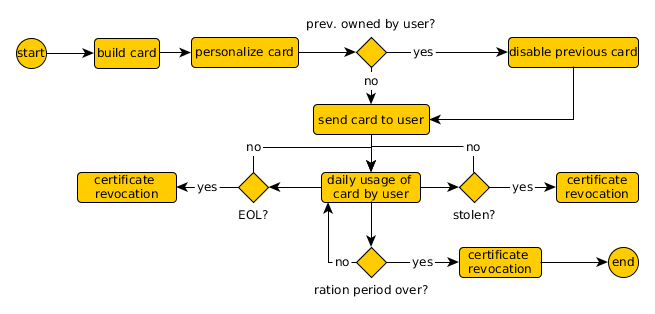
\includegraphics[width=0.8\textwidth]{lifecycle}
      \caption{The life-cycle of a petrol card in the PRS.}

\end{figure}

\end{itemize} % Usecases
\newpage
\section{Assets}
Our project case involves the following assets. Items enlisted with a * have not been implemented in the PRS due to time constraints and/or technical problems.
\begin{itemize}
\item Petrol

\item Petrol card
\begin{itemize}
 \item Card certificate, created with its own public and private keypair
 \item *Certificate from CA
 \item *\textcolor{red}{Signed timestamp of last requested revocation list received from CA}
 \item *\textcolor{red}{Timestamp indicating last charge}
 \item Current balance on the petrol card
% \item Card identification number
 \item PIN code
\end{itemize}

 \item Personalization terminals
 \begin{itemize}
 \item *\textcolor{red}{Terminal certificate, created with its own public and private keypair}
 \item Certificate from CA
 %\item Public and private key created for secure communication
% \item \textcolor{red}{TODO: check in code what other data is stored on IT}
 \item Terminal identification number
 \end{itemize}
 
 \item Charging terminals
 \begin{itemize}
    \item *\textcolor{red}{Terminal certificate, created with its own public and private keypair}
   	\item Certificate from CA
   	\item *\textcolor{red}{Signed timestamp of last requested revocation list received from CA}
 	\item Current monthly allowance that will be provided to all charging terminals
	\item List of revoked certificates
 \end{itemize}

 
 \item Petrol terminals
 \begin{itemize}
  	\item Terminal certificate, created with its own public and private keypair
  	\item Certificate from CA
 	\item  *\textcolor{red}{Signed timestamp of last requested revocation list received from CA}
 	\item List of revoked certificates
 \end{itemize}

 \item Back-end
 \begin{itemize}
 	\item Backend certificate, created with its own public and private key
 	\item Current monthly allowance that will be provided to all charging terminals
 	\item List of all generated certificates for terminals and petrol cards
 	\item List of revoked certificates
 	\item *The back-end will have a sub-CA certificate
 	\item *The main CA certificate will only be used to sign and revoke sub-CA certificates
 \end{itemize}
\end{itemize}

 % Assets
\section{Stakeholders}
The PRS has different stakeholders. The government is involved for the purpose of regulating the fuel consumption of the inhabitants. Petrol companies are involved for providing the fuel and for modifying their pumping installations to accommodate the PRS. They typically want low cost and low interaction/maintenance systems. The last stakeholder would be car owners, these are the end-users of the PRS and the owner of the petrol card. They typically want easy-to-use systems and a certain degree of privacy. 
 % Stakeholders
\section{Assumptions}
During the design of the PRS assumptions are made, these are listed below.
\begin{itemize}
\item Petrol card:\\
Every car owner will only have one petrol card. The petrol card is tamper-resistant, and therefore provides integrity and confidentiality to the data and functionality on the card, such as key material. Upon presenting a card to a terminal, the balance on the petrol card can only be modified by an authenticated charging terminal.  Petrol cards will automatically expire and revoked after 5 years.

\item Terminal: all terminals have a reliable clock. The key material and program code on the terminal cannot be copied or modified. The terminals are pre-installed at a secure location by screened personnel.

\item Personalization:\\
The code created for the PRS has been written by screened personnel and verified by various knowledgeable people whom have not detected backdoors in the code. %Employees working with the back-end or personalisation terminal do not have malicious intentions and have been properly instructed on how to use the system.

\item Charging:\\
The charging terminal will verify that the petrol balance is only increased once a month. 

\item Pumping:\\
The pump is trusted to always communicate the right amount of fuel that has been released to the pumping terminal. The pumping terminal is able to store logs of transactions without compromising the integrity or confidentiality of the logs.

\item Back-end:\\
The key material of the CA cannot be copied. The revocation list maintained by the back end cannot be altered in such a way that already revoked petrol cards or terminal will be removed from the revocation list. 
\end{itemize}

 
 % Assumptions
\section{Attacker model}
At any point in time it is likely that an attacker will try to perform an attack on the PRS. Likely adversaries for the PRS are: (organised) criminals, insiders and researchers. While most of the adversaries' capabilities, intentions and skills are alike, some may vary. Organised criminals are most likely to make money e.g. by obtaining and selling more petrol than rationed (or without collecting rations) and by obtaining legitimately issued petrol cards. To reach their goal they are more likely to take actions as extortion and violence. This group usually has the availability of large amounts of money to accomplish their goals. \\

Insiders have access or knowledge on the PRS and are familiar with the weak spots of the system. They will know or find ways to use this to their advantage. This group may try to bring down, or sabotage the workings of the system for a larger group of users. Attacks made by this group are likely to be accomplished with limited resources or money.  \\

Researchers are sometimes provided with full specifications on a system and  protocols. They are likely to break protocols such that they can intercept and manipulate any traffic between the petrol card and a terminal. This group will typically include researchers at an university, or a company hired to test the security of the system. The goals will be to break the security of the PRS in any way, which sometimes can result in a publication. This group usually has limited time and/or resources to accomplish their goals. 

Attacks by these adversaries can include, but are not limited to, MiTM, card tears and compromisation of key material. In case key material of a petrol card is compromised it should not bring down the PRS. An adversary will not be able to tamper with the petrol cards, nor will they be able to build a backdoor in the software of the terminals. 

%\textcolor{red}{All attackers have the possibility to perform a denial of service on the petrol cards, by THIS IS WHERE I LEFT OFF!..}

%This groups capabilities will include organised crime such as extortion and violence to obtain legitimately issued petrol cards. On the other hand it will also include card owners who may intentionally try to game the system by removing the petrol card from the terminal during a transaction. This group will mostly try to obtain more petrol than rationed.

%\end{itemize} %Attacker model

\section{Security requirements}
%\textcolor{red}{ALL REQUIREMENTS SHOULD BE CHECKED!}

% --- Start of the entire list ---
\begin{enumerate}
% --- Start of Confidentiality ---
\item Confidentiality
	\begin{enumerate}
%	\item The card identity number shall only be revealed to the  personalisation/charging/pump terminal after the terminal has been authenticated to the petrol card.
	\item The certificate and key material shall only be revealed to the IT/CT/PT after the terminal has been authenticated.
	\item The card usage shall not be revealed to any kind of terminal.
	\item The PIN code shall only be know by the petrol card and the petrol card owner. 
	\end{enumerate}
% --- End of Confidentiality ---
%\begin{minipage}{\linewidth}
% --- Start of Integrity ---
\item Integrity
	\begin{enumerate}
	\item The petrol balance on the petrol card can only be altered by an authenticated terminal.
	\item The identity number of the petrol card cannot be altered. 
	\item The certificate and key material on the petrol card and terminals cannot be altered.
	\item The logs on the terminal can only be altered by the terminal itself. 
	\item Communication between the terminals and back-end will be secure after they have both authenticated towards each other.
	\end{enumerate}
% --- End of Integrity ---
%\end{minipage}

% --- Start of Authentication ---
\item Authentication
		\begin{enumerate}
		\item The card owner shall authenticate to the CT or PT by entering the PIN to the petrol card.
	%	\item The charging terminal shall only receive the latest monthly petrol allowance after it has authenticate itself to the back-end %by means of certificates, \textcolor{red}{to receive the monthly petrol allowance that can be written to the petrol cards.REMOVE???}
		\item The back end will only provide the monthly allowance to the CT after it has authenticated itself.

		\item Communication between the terminals and back-end will be secure after they have both authenticated towards each other.
		\end{enumerate}	
		
%\item Authentication during pumping
%	\begin{enumerate}
%	\item The petrol card shall authenticate to the pumping terminal by using its public and private key. % providing its identity number (IDnr).
%	\item The pumping terminal shall authenticate itself to the petrol card by using its public and private keys
%	\item The pumping terminal shall authenticate itself to the back-end by using its public and private keys.

%	\end{enumerate}		
% --- End of Authentication ---

% --- Start of Authorisation ---
\item Authorisation
	\begin{enumerate}
	\item The CT is only authorised to update the petrol allowance to the petrol card once every month.
	\item The PT is authorised to withdraw petrol balance from the petrol card during a petrol transaction.
	\end{enumerate}
% --- End of Authorisation ---


% --- Start of Non-repudiation ---
\item Non-repudiation
	\begin{enumerate}
%		\item The petrol card shall obtain proof that the allowance value came from the back-end via the charging terminal.
%		\item The petrol card shall obtain proof that the changed allowance value came from the pumping terminal.
		\item The CT can prove to the back-end that it charged the monthly allowance to a valid petrol card. 
		\item The PT can prove to the back-end that it collected petrol allowance from a valid petrol card.
	\end{enumerate}
% --- End of Non-repudiation ---

\end{enumerate}
% --- End of the entire list ---
	%Security Requirements
\section{Design decisions}
During the design of the project, several design decisions were made, they are listed here.
\begin{itemize}
\item Petrol cards
\begin{itemize}
\item PIN code is used for authenticating the card owner to the terminals.
\item Public Key Infrastructure (PKI) is used for authentication, encryption and signatures of messages.
\item The petrol card will have an initial balance of zero once a car owner receives the petrol card. 
%\item All communications between petrol card and terminal are encrypted \& signed with a symmetric key. %except for the first communication of the certificate by either one party.
\item A symmetric key is used to secure communication between the petrol card and the terminal.
\item Petrol cards will have their own certificates and key material that will be initialised by the IT.
\end{itemize}

\item Terminal
\begin{itemize}
\item The IT will set the initial balance to zero.
\item The PIN codes will be set by the IT.
\item The CT will relay the signed allowance by the back end to the petrol card.
\item (*)A symmetric key is used to secure communication between the terminal and back-end. The SK is implemented, but allows the application to crash on some moments, we are unsure why this is the case. 
\item The petrol allowance on the petrol card can only be charged once a month.
\item The CT can see the petrol balance stored on the petrol card after the CT has authenticated itself to the petrol card.
\item The card owner will have to specify the required amount of petrol that he wishes to pump at the PT. In a previous design we planned on subtracting all balance from the petrol card. 
\end{itemize}


%\item Will ask for amount of fuel that is to be released. Card holder knows how much fuel is going to be used. Once entered, the card holder does not get rest of allowance back. So the pump terminal is not able to write allowance to the card.



%will the correct amount of used petrol Card owner will have to insert the petrol card into the petrol terminal for the whole transaction. The petrol terminal will receive the current petrol allowance on the card, the flow of petrol will be terminated if it reaches this number. If the petrol allowance is removed before the transaction is complete, the full petrol allowance will be removed upon the next presentation at a charging or petrol terminal. 

% until the fuel amount is chosen by the card owner. Petrol allowance on the card is provided to terminal, if the card is removed or this amount has been reached, the flow of petrol will be terminated. If the petrol card is removed during this moment, all petrol allowance will be removed from the card ???
%petrol allowance on the card will be decreased before its added to petrol terminal



\item Back-end
\begin{itemize}
\item *The back-end will sign and send the latest version of the CRL to the terminals
	%\item Will have a signed list of blocked petrol cards that are issued to the terminals.
%	\item Will have a list of all ID numbers belonging to each petrol card and terminal
%	\item Will have a sub-CA certificate, the utmost level in the certificate chain apart from the main CA.
%	\item The main CA certificate will only be used to sign and revoke sub-CA certificates
\end{itemize}
\end{itemize}

%\section{Overall design}
\subsection{PIN codes}
The user will have to enter a PIN code on the terminal numpad to verify ownership of the petrol card to the terminal. The terminal will send the PIN signed by its private key with the plain text of the PIN to the petrol card through the mutually authenticated encrypted channel. By which the petrol card will reply with whether the PIN number is correct or not. All specified functionality regarding PIN codes have been implemented. 

\subsection{Cryptography and PKI}
PKI is used to maintain and generate certificates. The back-end will operate as CA.  In the current situation the certificate of the main CA will be stored on a newly personalised petrol card. The back-end, terminals and petrol cards all have an RSA-1024 bit keypair. While this is not secure, nor recommended for long term use, it will suffice for testing and finding card limitations. The petrol card and terminals will receive a timestamp of the last update of certificate revocation list which is signed by the main CA certificate. This way it can be verified if the provided revocation list is recent. Each terminal will have the same setup: main CA certificate, its RSA keypair, and signed timestamp of the last updated certificate revocation list. \\

The CA certificate on each device is used to verify the validity and authenticity of each certificate during communication. Each end point, i.e petrol card and terminal, will verify the certificate of the other end point it is connecting to. In case the CA is notified of abuse or a breach, the certificate belonging to the end point will only be usable for 24 hours until the revocation list has been pushed to the end points. % At this point it is important to verify if the certificate has not been revoked by the CA. This way when the CA has been notified of abuse or breach in one of the end points, it will only take 24 hours for each end point to know of the revocation of a particular certificate. \\

Public and private keys in each end point will be used in conjunction with the CA certificate to mutually authenticate between each other. It is also used to negotiate an SK and also to provide integrity of the message by signing them. 

Due to time constraints and technical difficulties it was not possible to implement some aspects of the cryptography and PKI. To keep things simple for testing we created a CA, and not the sub-CA that would be used to sign all terminal and petrol certificates. Any signatures that we wanted to implement on revocation lists or messages were sadly not possible, since we were not able to get a certificate on the petrol card. The terminals and back-end do have their own certificate. We managed to get a SK to work between the petrol card and terminal, however sometimes this functionality gives an error and crashes the system, we are unsure why this happens.
%Due to technical issues it was not possible to implement the certificate on the petrol card, and thus signing the revocation list. 



 %A certificate consisting of a public and private key will be first created on the back-end (the overall system acting as the Certificate Authority). 

%\subsection{Public and Private keys in terminals/petrol cards}



\subsection{Protocol Descriptions}
\subsubsection{Mutual Authentication}
First the terminal sends a command APDU to enable the correct applet from the petrol card for the petrol rationing system. After that the terminal sends its certificate and public key to the petrol card. The petrol card verifies the certificate of the terminal and chooses a SK for encrypted communication. The petrol card signs its identification number with its private key, encrypts that signature and its own certificate with the SK. Then it sends the encrypted signature and certificate together with the SK encrypted by the public key of the terminal. Once the terminal receives the certificate of the petrol card, it verifies it. It then signs its own signature with its private key and combines this with a signed version of the identification number, encrypts them both with the SK and sends it to the petrol card.
\\

\begin{equation}\nonumber
\begin{split} 
T \to PC &: \text{commandAPDU to enable applet.}\\
T \to PC &: certificate_{T}, pub_{T}\\ 
PC &: \text{Verify}(certificate_{T}) \text{and choose SK}\\
PC \to T &: ENC_{SK}\{SIG[ID_{PC}]_{priv_{PC}}, certificate_{PC}\},  [SK]_{pub_T}\\
T&: \text{Verify}(certificate_{PC})\\
T \to PC &: ENC_{SK}\{SIG[ID_{T}]_{priv_T}, ID_{T}\} \\ 
\end{split} 
\end{equation}
and now we have a encrypted channel between a terminal and a petrol card.

\subsubsection{Certificate Validity Request}
After mutual authentication has been done, the petrol card will request the certificate revocation list from the terminal, who already has access the latest revocation list from the back-end. The revocation list is signed by the back-end. 

\begin{equation}\nonumber
\begin{split}
PC \to T &: [CVR + pub_{PC}]_{pub_{BE}}\\
T \to PC &: [SIG[VTS, TS, Certs]_{priv_{BE}}, VTS, TS, Certs]_{pub_{PC}}
\end{split} 
\end{equation}

\subsubsection{PIN validation and authentication of card owner}
After mutual authentication has been done, the terminal receives a PIN on the numpad from the card owner, signs the PIN and send the encryption of the signature with the plaintext PIN number to the petrol card. Once the petrol card receives the PIN number, returns the encrypted and signed boolean value (True/False) to the terminal after it verifies the PIN number. \\

PIN validation and authentication of card owner guarantees security requirement 1(d).

\begin{equation}\nonumber
\begin{split}
T \to PC&: ENC_{SK}\{SIG[PIN]_{priv_T}, PIN\}\\
PC \to T&: ENC_{SK}\{SIG[PIN_{AUTH}]_{priv_{PC}}, PIN_{AUTH}\}
\end{split} 
\end{equation}

\subsubsection{Getting petrol from the petrol terminal}
After mutual authentication and authentication of the card owner, the petrol card can send its current balance to the petrol terminal for getting petrol. The card owner will have to specify the amount of petrol he wishes to subtract from his balance. The PT will verify if this is possible and subtract this amount from the petrol card. After the transaction has been verified the PT will write a log entry with the time, identification number of the petrol card, balance and amount of  petrol that was pumped. If a card tear occurs the specified amount of petrol will be reduced from the petrol cards balance. We planned on adding something to this log that is signed by the card (such as balance and/or timestamp), however due to time constraints this was not implemented.  %Then, the terminal writes a balance of zero to the petrol card for cases where the card was removed mid transaction. Once the petrol has been pumped and the user successfully terminates the program, the terminal writes a new balance after deducting the pumped petrol amount from the initial balance sent by the card, to the card. And immediately after that the terminal logs the time, identification number, balance and the amount of petrol pumped by the user.

The terminal logging the timestamp, identification number and the balance before the petrol being pumped guarantees security requirement 5(b).

\begin{equation}\nonumber
\begin{split}
PC \to T&: ENC_{SK}\{SIG[B]_{priv_{PC}}, B\}\\
T&: \text{Log}(TS, ID_{PC}, B, SIG[TS, ID_{PC}, B]_{priv_T}) \\
T \to PC&: ENC_{SK}\{SIG[BZ]_{priv_T}, BZ\}\\
T&: \text{Calc}(B = B - UB)\\
T \to PC&: ENC_{SK}\{SIG[B]_{priv_T}, B\}\\
T&: \text{Log}(TS, ID_{PC}, B, UB, SIG[TS, ID_{PC}, B, UB]_{priv_T})
\end{split} 
\end{equation}


\subsubsection{Charging petrol allowance to the petrol card}
After mutual authentication, PIN validation and authentication of card owner
has been done, the petrol card can ask the charging terminal to charge its
allowed monthly petrol balance. Then the terminal starts a mutually
authenticated encrypted channel between itself and the back-end to get the monthly petrol allowance, and then
writes those values back to the petrol card.\\

The terminal starting a mutually authenticated encrypted channel with the back-end to get the monthly petrol allowance guarantees security requirement 1(e) \& 3(c).\\

The terminal logging the timestamp, identity number and the balance being written to the petrol card guarantees security requirement 6(a).

\begin{equation}\nonumber
\begin{split}
PC \to T&: \text{request APDU to initiate charging monthly allowance} \\
T&: \text{requests monthly allowance from back-end through the encrypted channel} \\
T&: \text{Log}(TS, ID_{PC}, B, SIG[TS, ID_{PC}, B]_{priv_T}) \\
T \to PC&: ENC_{SK}\{SIG[B,TS]_{priv_{BE}}, B, TS\}
\end{split} 
\end{equation}key material

\subsubsection{Invalidating petrol cards}
Petrol cards are invalidated by the back-end by means of revoking the certificate, which will be added to the revocation list. Cards can be added to the revocation list if the certificate is valid, if authentication of the user failed (incorrect PIN entry for three times), or any other suspicious behaviour. %\textcolor{red}{Possible other scenarios..}.

\subsubsection{States petrol card}
The petrol card can have both a transient and persistent state. The state diagrams for both states are showed in figure 2 and 3. The yellow boxes are the steps the petrol card will go through. The blue boxes are the variables that are recorded in the current state (thus EEPROM or RAM). 
%\textcolor{red}{TODO: explain how persistent and transient states are realised in the code }
\begin{figure}[!ht]
  \centering
    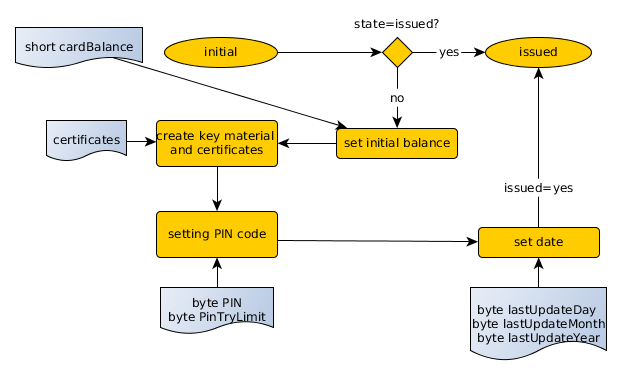
\includegraphics[width=0.7\textwidth]{persistant}
      \caption{The persistant states of the petrol card.}
\end{figure}

\begin{figure}[!ht]
  \centering
    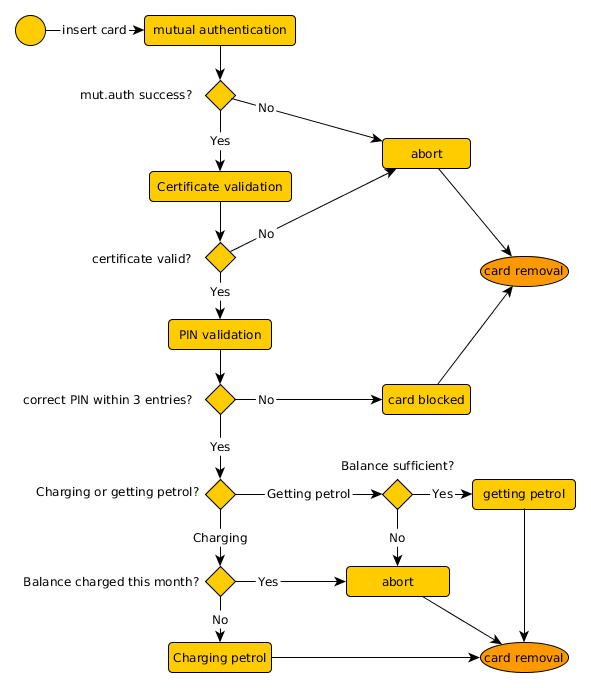
\includegraphics[width=0.7\textwidth]{transient}
      \caption{The transient states of the petrol card.}
\end{figure}	% Design decisions
%\section{Overall design}
\subsection{PIN codes}
The user will have to enter a PIN code on the terminal numpad to verify ownership of the petrol card to the terminal. The terminal will send the PIN signed by its private key with the plain text of the PIN to the petrol card through the mutually authenticated encrypted channel. By which the petrol card will reply with whether the PIN number is correct or not.

\subsection{Cryptography}
A certificate consisting of a public and private key will be first created on the back-end (the overall system acting as the Certificate Authority). Whenever a new petrol card is personalized, it will store the certificate of the main CA, create public and private key for itself and a timestamp of the last update of certificate revocation list which is signed by the main CA certificate. Each terminal will have the same setup: main CA certificate, its own public and private key, and signed timestamp of the last updated certificate revocation list.

\subsection{CA certificate stored in terminals/petrol cards}
The main certificate from the CA stored in each terminal and petrol card is used to verify the validity and authenticity of each certificate during communication. Each end point, i.e both petrol card and terminal alike, will verify the certificate of the other end point it is connecting to, whether the certificate has been revoked or not by the CA. This way when the CA has been notified of abuse or breach in one of the end points, it will only take 24 hours for each end point to know of the revocation of a particular certificate.

\subsection{Public and Private keys in terminals/petrol cards}
Public and private keys in each end point will be used in conjunction with the CA certificate to mutually authenticate between each other. It is also used to negotiate a SK and also to provide integrity of the message by signing them.


\subsection{Protocol Descriptions}



\subsubsection{Mutual Authentication}
First the terminal sends a command APDU to enable the correct applet from the petrol card for the petrol rationing system. After that the terminal sends its certificate and public key to the petrol card. The petrol card verifies the certificate of the terminal and chooses a SK for encrypted communication. The petrol card signs its identification number with its private key, encrypts that signature and its own certificate with the SK. Then it sends the encrypted signature and certificate together with the SK encrypted by the public key of the terminal. Once the terminal receives the certificate of the petrol card, it verifies it. It then signs its own signature with its private key and combines this with a signed version of the identification number, encrypts them both with the SK and sends it to the petrol card.
\\

\begin{equation}\nonumber
\begin{split} 
T \to PC &: \text{commandAPDU to enable applet.}\\
T \to PC &: certificate_{T}, pub_{T}\\ 
PC &: Verify(certificate_{T}) \text{and choose SK}\\
PC \to T &: ENC_{SK}\{SIG[ID_{PC}]_{priv_{PC}}, certificate_{PC}\},  [ENC_{SK}]_{pub_T}\\
T&: Verify(certificate_{PC})\\
T \to PC &: ENC_{SK}\{SIG[ID_{T}]_{priv_T}, ID_{T}\} \\ 
\end{split} 
\end{equation}
and now we have a encrypted channel between a terminal and a petrol card.

\subsubsection{Certificate Validity Request}
After mutual authentication has been done, the petrol card will request the certificate revocation list from the back-end through the terminal. In this case, the terminal just acts as a relay between the petrol card and the back-end.

\begin{equation}\nonumber
\begin{split}
PC \to BE &: [CVR + pub_{PC}]_{pub_{BE}}\\
BE \to PC &: [SIG[VTS, TS, Certs]_{priv_{BE}}, VTS, TS, Certs]_{pub_{PC}}
\end{split} 
\end{equation}
\subsubsection{PIN validation and authentication of card owner}
After mutual authentication has been done, the terminal receives a PIN on the numpad from the card owner, signs the PIN and send the encryption of the signature with the plaintext PIN number to the petrol card. Once the petrol card receives the PIN number, returns the encrypted and signed boolean value (True/False) to the terminal after it verifies the PIN number. \\

PIN validation and authentication of card owner guarantees security requirement 1(d).

\begin{equation}\nonumber
\begin{split}
T \to PC&: ENC_{SK}\{SIG[PIN]_{priv_T}, PIN\}\\
PC \to T&: ENC_{SK}\{SIG[PIN_{AUTH}]_{priv_{PC}}, PIN_{AUTH}\}
\end{split} 
\end{equation}

\subsubsection{Getting petrol from the petrol terminal}
After mutual authentication, PIN validation and authentication of card owner has been done, the petrol card can send its current balance to the petrol terminal for getting petrol. Then, the terminal writes a balance of zero to the petrol card for cases where the card was removed mid transaction. Once the petrol has been pumped and the user successfully terminates the program, the terminal writes a new balance after deducting the pumped petrol amount from the initial balance sent by the card, to the card. And immediately after that the terminal logs the time, identification number, balance and the amount of petrol pumped by the user.

The terminal logging the timestamp, identification number and the balance before the petrol being pumped guarantees security requirement 6(b).

\begin{equation}\nonumber
\begin{split}
PC \to T&: ENC_{SK}\{SIG[B]_{priv_{PC}}, B\}\\
T&: Log(TS, ID_{PC}, B, SIG[TS, ID_{PC}, B]_{priv_T}) \\
T \to PC&: ENC_{SK}\{SIG[BZ]_{priv_T}, BZ\}\\
T&: Calc(B = B - UB)\\
T \to PC&: ENC_{SK}\{SIG[B]_{priv_T}, B\}\\
T&: Log(TS, ID_{PC}, B, UB, SIG[TS, ID_{PC}, B, UB]_{priv_T})
\end{split} 
\end{equation}


\subsubsection{Charging petrol allowance to the petrol card}
After mutual authentication, PIN validation and authentication of card owner
has been done, the petrol card can ask the charging terminal to charge its
allowed monthly petrol balance. Then the terminal starts a mutually
authenticated encrypted channel between itself and the back-end to get the monthly petrol allowance, and then
writes those values back to the petrol card.\\

The terminal starting a mutually authenticated encrypted channel with the back-end to get the monthly petrol allowance guarantees security requirement 1(e) \& 3(c).\\

The terminal logging the timestamp, identity number and the balance being written to the petrol card guarantees security requirement 6(a).

\begin{equation}\nonumber
\begin{split}
PC \to T&: \text{request APDU to initiate charging monthly allowance} \\
T&: \text{requests monthly allowance from back-end through the encrypted channel} \\
T&: Log(TS, ID_{PC}, B, SIG[TS, ID_{PC}, B]_{priv_T}) \\
T \to PC&: ENC_{SK}\{SIG[B,TS]_{priv_{BE}}, B, TS\}
\end{split} 
\end{equation}
 %Overall design
%\input{organisation}\newpage
%\input{reflection}

%{} sym
%[] pub
\end{document}
